\documentclass[oneside,14pt]{extarticle}
\usepackage[utf8]{inputenc}
\usepackage[english,ukrainian]{babel}
\usepackage{amssymb,amsfonts,amsmath,amsthm,mathtext,textcomp}

\usepackage[includehead, headsep=0pt, footskip=0pt, top=2cm, bottom=2cm, left=2cm, right=1cm]{geometry}
\usepackage{indentfirst}
\usepackage[onehalfspacing]{setspace}
\usepackage[headings]{fancyhdr}
\usepackage{etoolbox}
\usepackage{flafter}
\usepackage{listings}
\usepackage{graphicx}
\usepackage{float}
\usepackage[labelsep=period]{caption}
\lstset{
	breaklines=false
}
\usepackage{array}
\fancyhf{}
\renewcommand{\headrulewidth}{0pt}
\pagestyle{fancy}
\fancyfoot[R]{\thepage}
\lstset{breaklines=true,}
\graphicspath{ {./pictures} }

\lstset{
	language=c,
	tabsize=4,
	keepspaces,
	showstringspaces=false,
}
\graphicspath{ {./pictures} }
\setlength{\parindent}{4em}
\setlength\tabcolsep{5px}

\newcommand\subject{Моделювання та аналіз програмного забезпечення}
\newcommand\lecturer{доцент кафедри ПЗ \\ Сердюк П.В.}
\newcommand\teacher{викладач кафедри ПЗ \\ Микуляк А.В.}
\newcommand\mygroup{ПЗ-22}
\newcommand\lab{3}
\newcommand\theme{Твірні шаблони проектування}
\newcommand\purpose{Здобути навички використання твірних шаблонів проектування при моделюванні програмних систем}

\begin{document}
\begin{normalsize}
	\begin{titlepage}
		\thispagestyle{empty}
		\begin{center}
			\textbf{МІНІСТЕРСТВО ОСВІТИ І НАУКИ УКРАЇНИ\\
				НАЦІОНАЛЬНИЙ УНІВЕРСИТЕТ "ЛЬВІВСЬКА ПОЛІТЕХНІКА"}
		\end{center}
		\begin{flushright}
			\textbf{ІКНІ}\\
			Кафедра \textbf{ПЗ}
		\end{flushright}
		\vspace{70pt}
		\begin{center}
			\textbf{ЗВІТ}\\
			\vspace{10pt}
			до лабораторної роботи № \lab\\
			\textbf{на тему}: “\textit{\theme}”\\
			\textbf{з дисципліни}: “\subject”
		\end{center}
		\vspace{50pt}
		\begin{flushright}
			
			\textbf{Лектор}:\\
			\lecturer\\
			\vspace{10pt}
			\textbf{Виконав}:\\
			
			студент групи \mygroup\\
			Коваленко Д.М.\\
			\vspace{10pt}
			\textbf{Прийняв}:\\
			
			\teacher\\
			
			\vspace{28pt}
			«\rule{1cm}{0.15mm}» \rule{1.5cm}{0.15mm} 2023 р.\\
			$\sum$ = \rule{1cm}{0.15mm}……………\\
			
		\end{flushright}
		\vspace{\fill}
		\begin{center}
			\textbf{Львів — 2023}
		\end{center}
	\end{titlepage}
		
	\begin{description}
		\item[Тема.] \theme.
		\item[Мета.] \purpose.
	\end{description}

	\section*{Завдання}
Розробити твірні шаблони проектування відповідно до прецедентів обраного варіанту
ігрової логіки. Вибрати один з прецедентів, для якого найбільш доцільно застосувати твірний
шаблон (не всі прецеденти цього потребуватимуть).

	Представити діаграму класів ігрового проекту (із відображенням на ній використаних
	шаблонів).

	\section*{Хід виконання}
	
	\begin{figure}[H]
		\centering
		\includegraphics[]{singleton}
		\caption{UML діаграма реалізації шаблону Singleton}
	\end{figure}
	
	\begin{figure}[H]
		\centering
		\includegraphics[]{singleton-ex}
		\caption{UML діаграма прикладу реалізації шаблону Singleton}
	\end{figure}
	
	\begin{small}
		\begin{lstlisting}
export class GameState {
	private static instance: GameState;
	private state: State;
	
	private constructor() {
		this.state = State.Playing;
	}
	
	public static getInstance(): GameState {
		if (!GameState.instance) {
			GameState.instance = new GameState();
		}
		return GameState.instance;
	}
	
	public getState(): State {
		return this.state;
	}
	
	public setState(state: State): void {
		this.state = state;
	}
}
		\end{lstlisting}
	\end{small}
	
	\begin{figure}[H]
		\centering
		\includegraphics[width=\textwidth]{abstract-factory}
		\caption{UML діаграма реалізації шаблону Abstract Factory}
	\end{figure}
	
		\begin{figure}[H]
		\centering
		\includegraphics[width=\textwidth]{abstract-factory-ex}
		\caption{UML діаграма прикладу реалізації шаблону Abstract Factory}
	\end{figure}
	
	\begin{small}
		\begin{lstlisting}
export interface AlienFactory {
	createAlien(scene: Phaser.Scene, x: number, y: number): Alien;
}

export class Type1AlienFactory implements AlienFactory {
	createAlien(scene: Phaser.Scene, x: number, y: number): AlienT1 {
		return new AlienT1(scene, x, y);
	}
}

export class Type2AlienFactory implements AlienFactory {
	createAlien(scene: Phaser.Scene, x: number, y: number): AlienT2 {
		return new AlienT2(scene, x, y);
	}
}
		\end{lstlisting}
	\end{small}
	
	\begin{figure}[H]
		\centering
		\includegraphics[]{factory}
		\caption{UML діаграма реалізації шаблону Factory}
	\end{figure}
	
		\begin{figure}[H]
		\centering
		\includegraphics[width=\textwidth]{factory-ex}
		\caption{UML діаграма прикладу реалізації шаблону Factory}
	\end{figure}
	
	\begin{small}
		\begin{lstlisting}
export class BulletFactory {
	private scene: Phaser.Scene;
	
	constructor(scene: Phaser.Scene) {
		this.scene = scene;
	}
	
	createBullet(): Bullet {
		return new Bullet(this.scene);
	}
}
		\end{lstlisting}
	\end{small}
	
	\begin{figure}[H]
		\centering
		\includegraphics[]{builder}
		\caption{UML діаграма реалізації шаблону Builder}
	\end{figure}
	
	\begin{figure}[H]
		\centering
		\includegraphics[]{builder-ex}
		\caption{UML діаграма прикладу реалізації шаблону Builder}
	\end{figure}
	
	\begin{small}
		\begin{lstlisting}
export class Ship {
	private x: number;
	private y: number;
	private collideWorldBounds: boolean;
	
	constructor() {
		this.x = 400;
		this.y = 500;
		this.collideWorldBounds = true;
	}
	
	setX(x: number): Ship {
		this.x = x;
		return this;
	}
	
	setY(y: number): Ship {
		this.y = y;
		return this;
	}
	
	setCollideWorldBounds(collide: boolean): Ship {
		this.collideWorldBounds = collide;
		return this;
	}
	
	build(scene: Phaser.Scene): Phaser.Physics.Arcade.Sprite {
		let ship = scene.physics.add.sprite(this.x, this.y, AssetType.Ship);
		ship.setCollideWorldBounds(this.collideWorldBounds);
		return ship;
	}
	
	static create(): Ship {
		return new Ship();
	}
}
		\end{lstlisting}
	\end{small}
	
	\begin{figure}[H]
		\centering
		\includegraphics{prototype}
		\caption{UML діаграма реалізації шаблону Prototype}
	\end{figure}
	
		\begin{figure}[H]
		\centering
		\includegraphics{prototype-ex}
		\caption{UML діаграма прикладу реалізації шаблону Prototype}
	\end{figure}
	
	\begin{small}
		\begin{lstlisting}
export class EnemyBullet extends Phaser.Physics.Arcade.Sprite {
	constructor(scene: Phaser.Scene) {
		super(scene, 0, 0, AssetType.EnemyBullet);
	}
	
	clone(): EnemyBullet {
		return new EnemyBullet(this.scene);
	}
	
	kill() {
		this.destroy();
	}
}
		\end{lstlisting}
	\end{small}
	
	\begin{figure}[H]
		\centering
		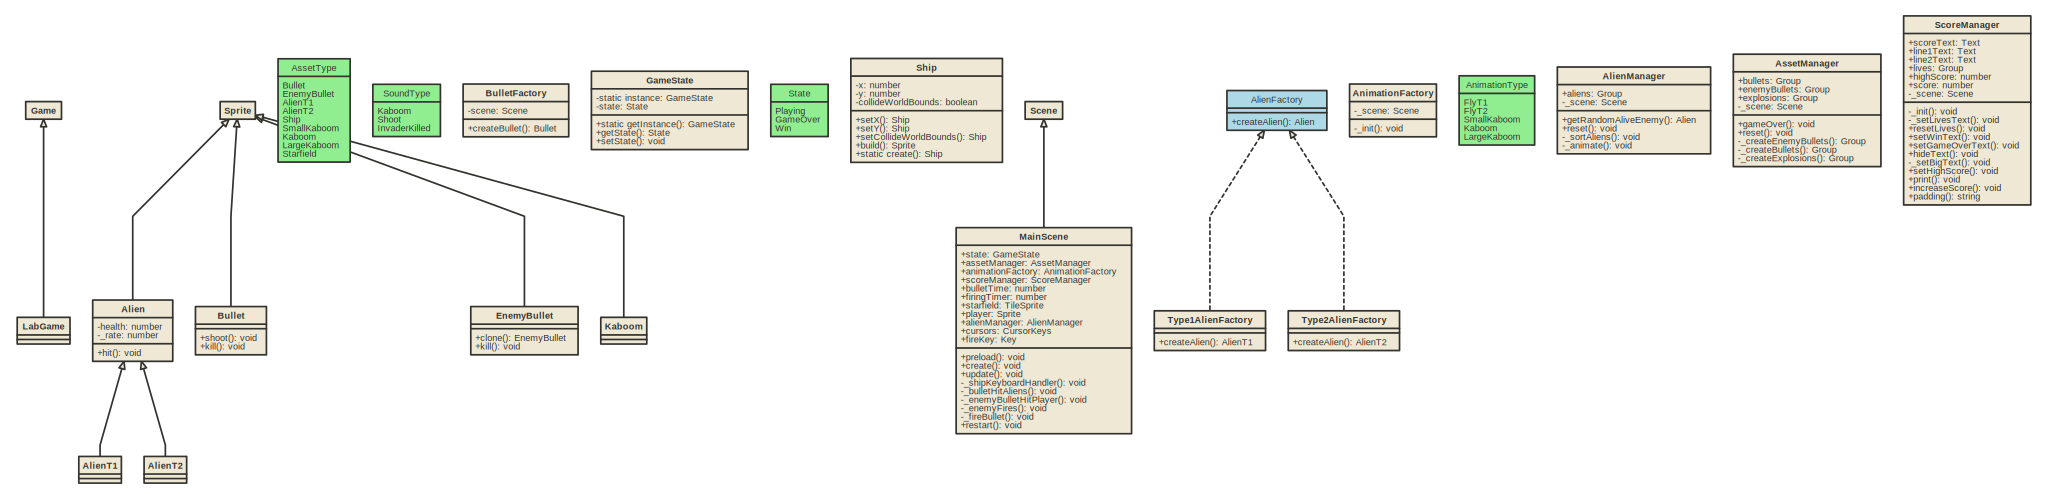
\includegraphics[width=\textwidth]{out}
		\caption{UML діаграма усього проекту}
	\end{figure}
	
	\section*{Висновки}
	   Під час виконання лабораторної роботи я здобув навички використання твірних шаблонів проектування при моделюванні програмних систем.
\end{normalsize}
\end{document}
